\section{系统设计}\label{sec:SystemDesign}

在本节(\cref{sec:SystemDesign})中,笔者将详细探讨 MinmusOS 项目的系统设计原则、系统架构设计、系统技术选型,以及项目结构设计。系统设计原则是确保操作系统可靠性、效率和可维护性的基础,包括封装、高内聚低耦合、面向对象设计、异常处理等多个方面。系统架构设计则涵盖了操作系统的主要组成部分,如引导程序、内核、标准运行库和应用程序,每个部分的功能和设计细节将在后文中详细阐述。系统技术选型将解释为何选择特定的编程语言和硬件架构对于 MinmusOS 的开发至关重要,特别是选择 Rust 语言而不是传统的 C/C++,以及选择基于 IA-32 架构的硬件平台的原因。这些技术选型不仅反映了对现有技术和资源的最大利用,也展示了项目在安全性和性能优化方面的考量。项目结构设计部分将介绍 MinmusOS 的组织结构,包括代码的模块化布局和各组件之间的交互方式,以确保高效的开发和维护流程。

\subsection{系统设计原则}

MinmusOS 的系统设计遵循了多个重要的软件工程原则,以确保其健壮性、可维护性和效率。

\subsubsection{封装(Encapsulation)}

在 MinmusOS 中,封装是通过模块化设计实现的,每个模块负责特定的功能。例如,内核中的驱动程序模块、内存管理模块、文件系统模块等,每个模块都将其内部数据和实现细节隐藏起来,只通过定义良好的接口与外界交互。这种封装确保了模块之间的依赖性最小化,同时也便于每个模块独立更新和维护。

\subsubsection{高内聚低耦合(High Cohesion and Low Coupling)}

MinmusOS 严格执行高内聚低耦合的设计原则。每个模块(如内存管理、进程调度等)都专注于一个具体的任务,确保模块内部各个部分紧密相关,共同完成单一功能,即高内聚。模块之间的交互通过简洁的接口进行,减少了依赖性。例如,内核与用户应用通过系统调用接口通信,系统调用接口提供了一个抽象层,使得用户程序不需要关心具体的硬件细节,即低耦合。

\subsubsection{面向对象(Object-Oriented)}

尽管 MinmusOS 主要用 Rust 实现,它仍然采用了面向对象的设计原则。各种硬件驱动程序可能继承自一个通用的驱动程序接口,实现特定的接口函数,这支持了代码的重用和模块间的互操作性。

\subsubsection{异常处理(Exception Handling)}

MinmusOS 通过全面的异常处理机制来增强系统的稳定性和安全性。内核设计包括对硬件和软件异常的捕获和处理,如中断、页错误和其他 CPU 异常。通过定义异常处理程序,系统能够优雅地响应未预料的事件,保证系统的连续运行或安全地失败。

\subsubsection{维护性(Maintainability)}

系统的设计允许容易地添加新功能或修改现有功能而不影响其他部分。通过使用版本控制系统(Git),MinmusOS 的维护和更新变得更加高效。代码的组织和文档化也支持快速理解和问题定位。

\subsubsection{模块性(Modularity)}

MinmusOS 的模块性设计允许系统被划分为多个独立的部分,每个部分承担特定的职责。这种设计不仅使得各个模块可以独立开发、测试和维护,而且通过定义清晰的接口,减少了模块间的依赖关系,提高了整个系统的灵活性和可维护性。

\subsubsection{扩展性(Scalability)}

MinmusOS 在设计时考虑到了扩展性,确保系统可以随着需求的增长而适应。系统支持动态加载和卸载功能模块,允许用户根据需要调整系统配置和资源利用,从而在用户和功能数量增加时仍能保持良好的性能和响应速度。

\subsubsection{安全性(Security)}

安全性是 MinmusOS 设计的核心之一,系统采用多种机制确保运行的安全。利用 Rust 语言的内存安全特性,系统有效防止了内存泄漏和越界错误。此外,通过实施严格的访问控制和使用最小权限原则,MinmusOS 保护系统免受未授权访问和潜在的恶意攻击。

\subsection{系统架构设计}

MinmusOS 主要由四个模块组成:引导程序(Bootloader)、内核(Kernel)、标准运行库(Standard Runtime Library)和应用程序(Applications):

\begin{enumerate}
    \item \textbf{引导程序(Bootloader)}:MinmusOS的引导程序负责系统启动的初始阶段。它首先在实模式下运行,设置必要的环境后转入保护模式。
          \begin{enumerate}
              \item \textbf{主引导记录}:存储在硬盘的第一个扇区,负责加载引导程序的其余部分。MBR还包含了分区表,指明硬盘的分区信息。
              \item \textbf{BIOS中断}:利用BIOS提供的中断调用来实现基本的输入输出系统功能,如读取磁盘数据和显示信息。
              \item \textbf{磁盘读取器}:一个专门的模块,用于从磁盘读取操作系统的内核数据到内存。
              \item \textbf{实模式}:CPU的一种操作模式,允许引导程序访问系统的基础硬件资源,如内存和I/O端口。
              \item \textbf{保护模式}:引导程序将系统从实模式切换到保护模式以支持更高级的功能,如虚拟内存和多任务处理。
              \item \textbf{全局描述符表}:在保护模式下使用,用于定义不同的内存段,如代码段和数据段。
              \item \textbf{打印器}:在系统启动过程中用于输出调试信息到屏幕或其他输出设备。
          \end{enumerate}
    \item \textbf{内核(Kernel)}:MinmusOS的内核是系统的核心,处理所有基本的系统任务,如进程管理、内存管理和设备驱动。
          \begin{enumerate}
              \item \textbf{中断}:处理硬件和软件中断,使内核能响应外部事件,如硬件信号或软件异常。
              \item \textbf{驱动程序}:内核包含各种设备驱动程序,使其能够控制和管理硬件设备。
              \item \textbf{多任务处理}:实现进程调度和管理,允许多个程序并发运行,优化CPU使用。
              \item \textbf{系统调用}:提供一个接口供应用程序请求内核服务,如文件操作和进程管理。
              \item \textbf{VGA文本模式}:利用VGA硬件实现文本输出,用于显示系统信息和用户界面。
              \item \textbf{内存管理}:包括虚拟内存管理和物理内存分配,确保有效利用内存资源。
              \item \textbf{文件系统}:实现文件的存储、检索和管理,支持数据的持久化。
              \item \textbf{定时器}:提供计时功能,支持操作系统和应用程序的时间管理需求。
              \item \textbf{命令行解释器}:允许用户通过命令行界面与系统交互,执行各种命令。
          \end{enumerate}
    \item \textbf{标准运行库(Standard Runtime Library)}:标准运行库提供一组基础库和工具,支持内核和应用程序的运行。
          \begin{enumerate}
              \item \textbf{math库}:支持各种数学运算,如加减乘除和三角函数。
              \item \textbf{mutex库}:实现互斥锁,支持多线程或多进程间的同步。
              \item \textbf{print库}:提供基本的文本输出功能,用于在终端或其他设备上显示信息。
              \item \textbf{rand库}:包含多种随机数生成方法,为系统和应用程序提供随机性支持
              \item \textbf{sort库}:实现各种排序算法,如快速排序和归并排序,供程序处理数据时使用。
              \item \textbf{string库}:提供字符串处理功能,如字符串拼接、分割和搜索。
          \end{enumerate}
    \item \textbf{应用程序(Applications)}:MinmusOS支持用户编写和运行应用程序。系统提供了一套应用程序编程接口(API),以及用于编译和链接应用程序的脚本。应用程序可以直接使用内核提供的系统调用,以及标准运行库中的功能。
\end{enumerate}

\label{fig:SystemArchitecture}展示了MinmusOS的系统架构。

此架构设计旨在提供一个模块化和可扩展的操作系统,每个部分都有明确的职责,相互协作以提供高效稳定的系统运行。

\begin{figure}[htbp]
    \centering
    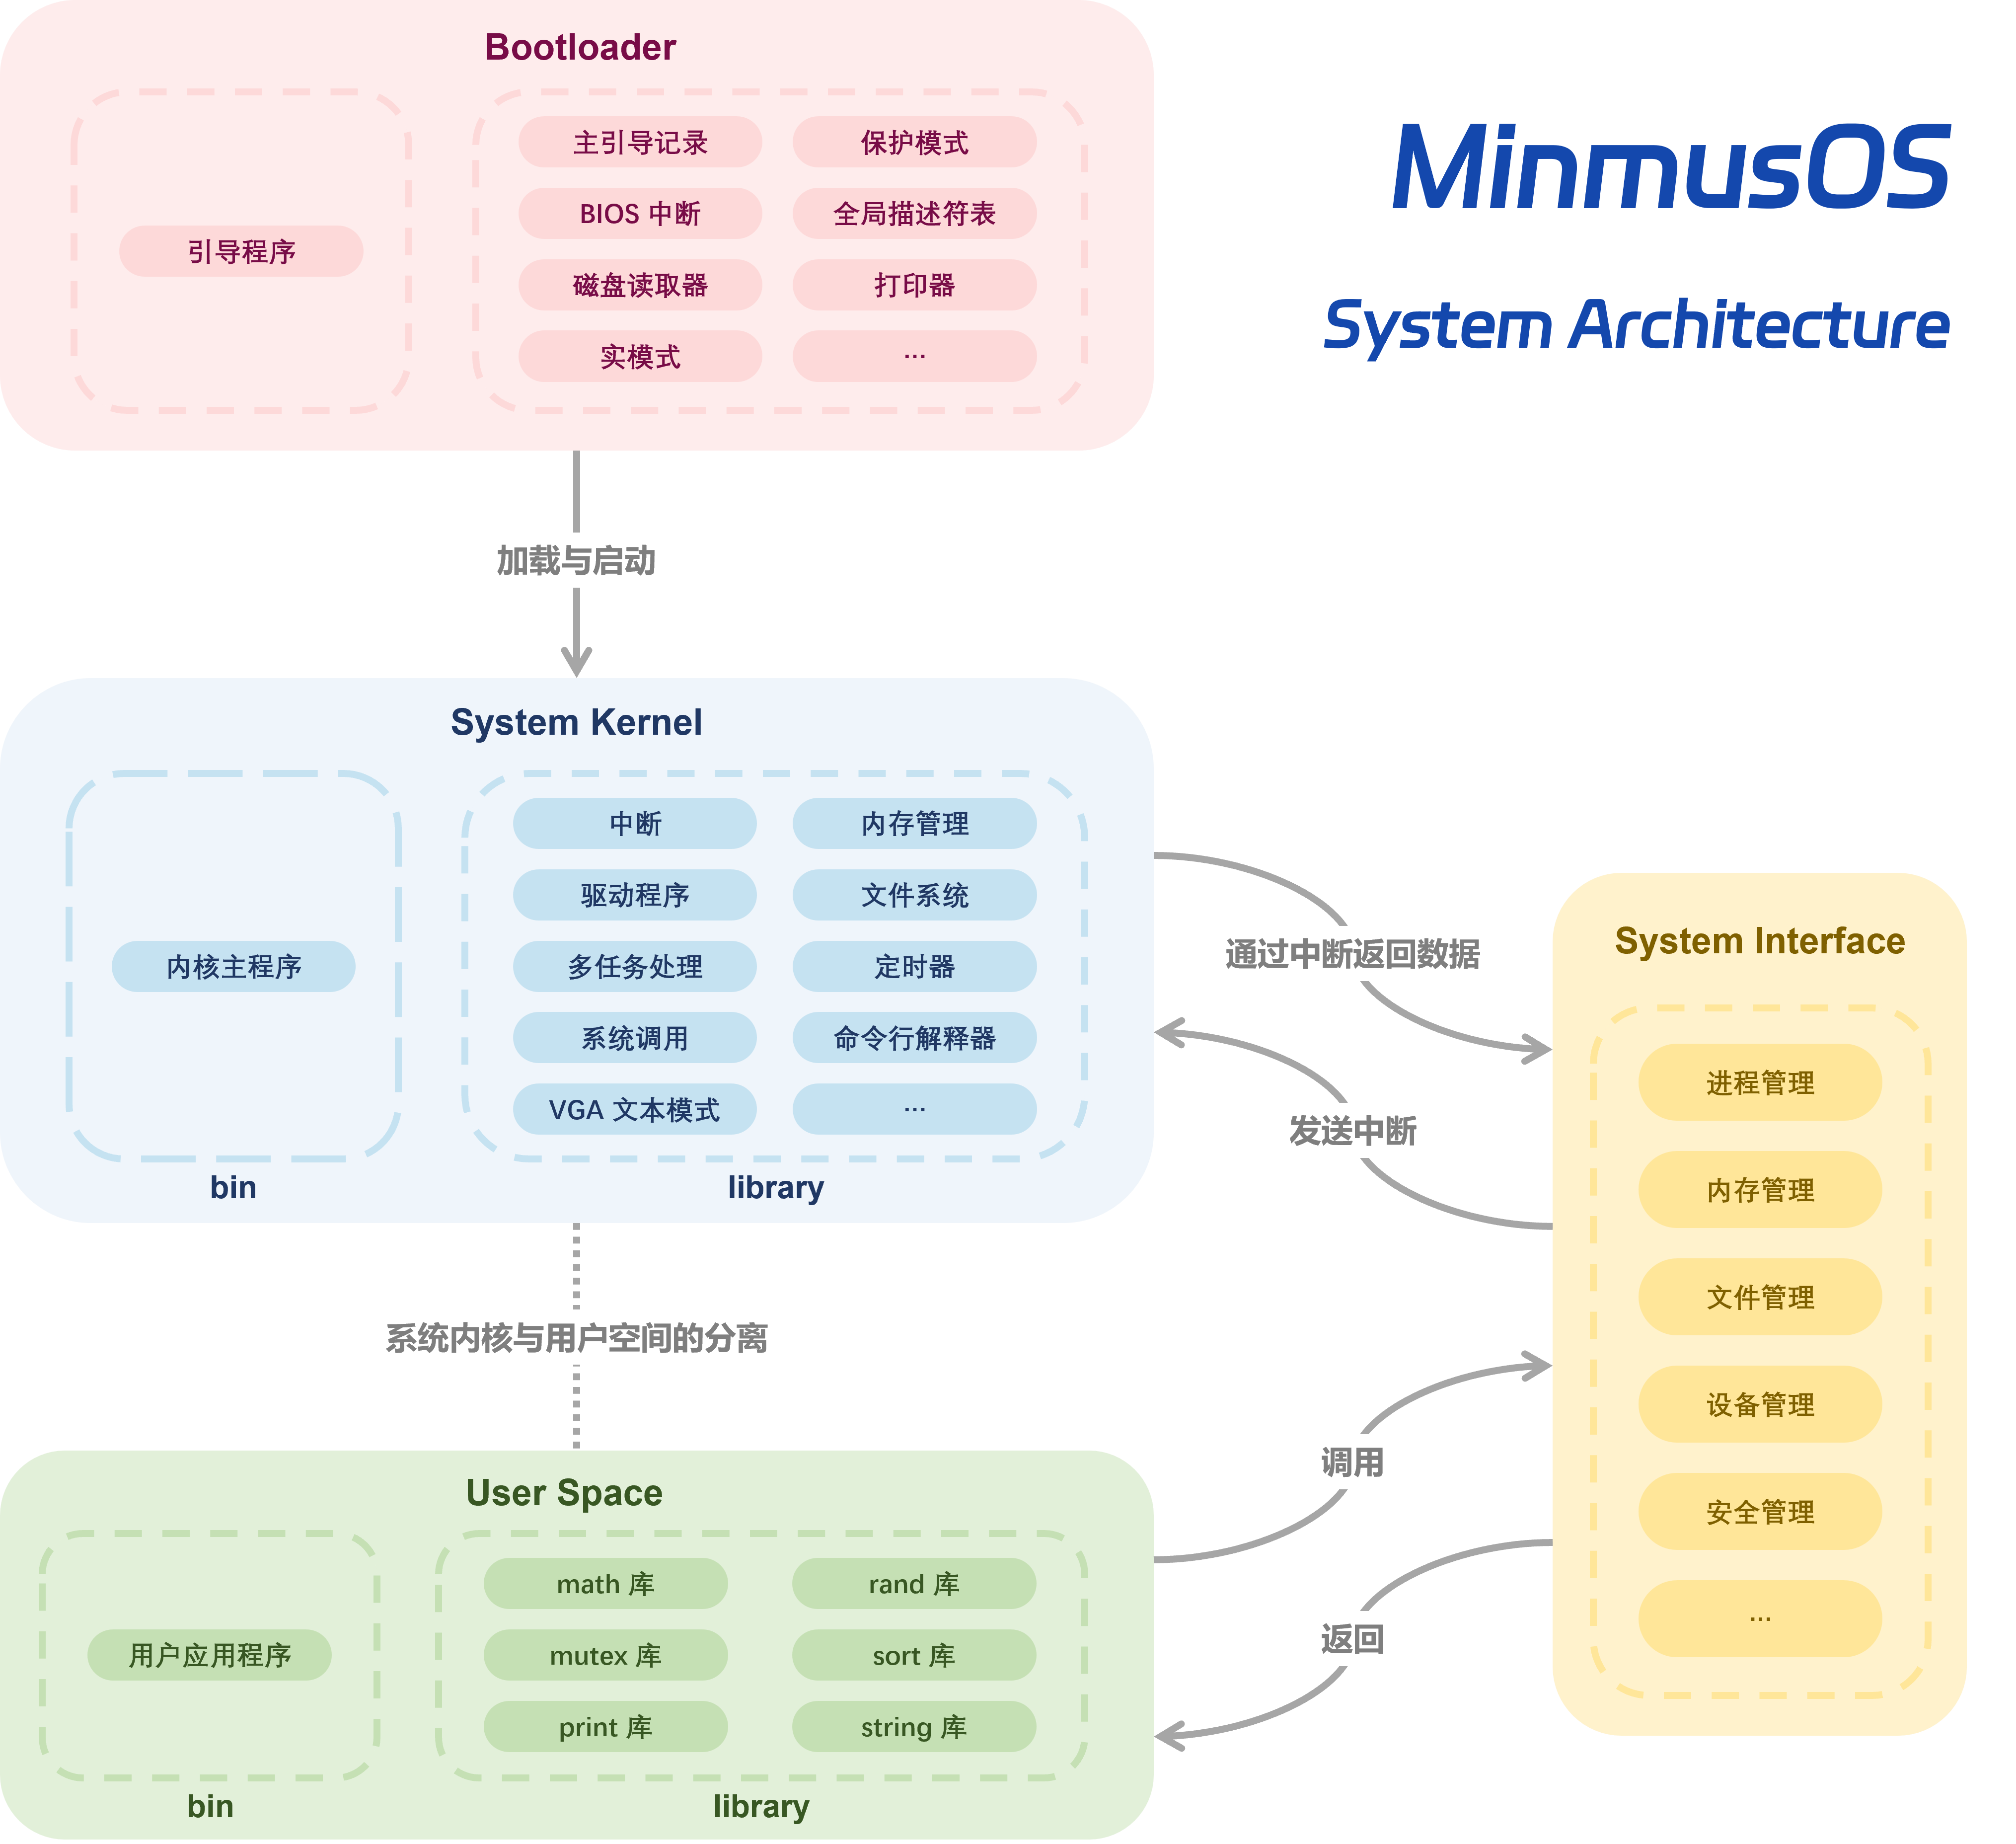
\includegraphics[width=\textwidth]{figures/SystemArchitecture.png}
    \caption{MinmusOS系统架构}
    \label{fig:SystemArchitecture}
\end{figure}

\subsection{系统技术选型}\label{sec:SystemTechnicalSelection}

\subsubsection{编程语言}

本系统选择Rust作为编程语言,而不选择C/C++编程语言。

\paragraph{C/C++语言在操作系统开发中的传统地位}

C 语言自 1972 年诞生以来,由于其接近硬件的编程能力和高效的性能表现,迅速成为操作系统开发的首选语言。最著名的例子是 Unix 操作系统,它几乎完全用 C 语言编写,此后引发了包括 Linux、Windows 和 macOS 在内的多个主流操作系统的开发倾向。这种历史悠久的使用背景为 C 语言在操作系统领域内奠定了坚实的基础,使其成为系统级编程的标准工具。

C 语言的主要技术优势在于其提供了极大的硬件操作能力和控制精度。开发者可以直接管理内存地址和硬件资源,这对于实现低级别的操作系统功能至关重要。此外,C 语言拥有强大的编译器优化能力,能够生成高效的机器代码,最大限度地提高运行时性能。

C 语言还受益于广泛的工具链支持,包括各种编译器(如 GCC 和 Clang)、调试工具(如 GDB)以及大量的库和开发资源。这些工具和资源的成熟与丰富,为操作系统开发提供了必要的技术支持和社区帮助。

C++ 作为 C 语言的后继者,最早于 1983 年由 Bjarne Stroustrup 开发,它在 C 语言的基础上增加了面向对象编程、泛型编程和其他高级特性。C++ 保留了 C 语言的硬件操作能力和性能,同时引入了类、继承和多态等面向对象的概念,使得开发者可以更好地组织和管理复杂的系统。

在操作系统开发中,C++ 提供了更高的抽象能力,使代码的可读性和可维护性得以提高。例如,Windows 内核在某些模块中就使用了 C++ 语言来实现,以便利用其面向对象的特性来组织复杂的系统组件和服务。同时,C++ 提供了强大的标准库(STL),这为开发过程中常见的数据结构和算法提供了开箱即用的实现,进一步提高了开发效率。

\paragraph{C语言在操作系统开发中的劣势}

尽管 C 语言在操作系统开发中具有显著的优势,但它也存在一些不可忽视的劣势。其中最为人所诟病的是内存安全问题,包括内存泄漏、野指针和缓冲区溢出等,这些问题常常导致系统的不稳定甚至安全漏洞。同时,C 语言在并发和并行处理方面的支持较为原始,缺乏现代编程语言中常见的高级并发控制机制,这在多核处理器日益普及的今天显得尤为突出。

\subparagraph{内存管理问题}

在 C 语言中,内存管理完全依赖于程序员的手动控制,包括内存的分配与释放。这种管理方式虽然提供了最大程度的控制,但同时也引入了诸多潜在问题,如内存泄漏、野指针、内存碎片以及空指针访问等。这些问题不仅增加了编程的复杂性,还可能导致程序运行时出现严重的稳定性和安全性问题。例如,忘记释放内存会造成内存泄漏,而错误地访问已释放的内存(悬垂指针)则可能导致不可预测的程序行为或系统崩溃。

\subparagraph{类型安全和数据完整性问题}

C 语言的类型系统允许隐式类型转换和直接的指针运算,这虽然在某些情况下提供了便利,但也容易导致类型安全问题。例如,一个整数可以无警告地转换为较小的数据类型,造成数据溢出;指针类型之间也可以轻易地转换,增加了非法内存访问的风险。这种类型系统的松散性能够导致数据损坏、程序错误和安全漏洞。

\subparagraph{封装性和模块化的不足}

C 语言作为一种面向过程的编程语言,缺乏现代面向对象语言所提供的类、继承和多态等封装和抽象机制。虽然可以通过结构体和函数指针等手段模拟一些面向对象的功能,但这种做法通常较为笨拙且效率不高。缺乏高级的封装机制,使得在大型项目中实现代码的模块化和复用变得更加困难,从而影响了代码的可维护性和可扩展性。

\subparagraph{使用外部库的挑战}

尽管 C 语言拥有大量的第三方库,但缺乏一个统一的、官方支持的包管理系统,使得管理和维护这些库变得复杂。程序员需要手动管理库的依赖关系、编译配置和命名冲突,这不仅增加了使用外部资源的门槛,也可能引入版本不一致等问题。

\subparagraph{异常处理的缺失}

C 语言没有内置的异常处理机制。错误通常通过返回码来标示,或者使用全局变量来记录错误状态。这种方式要求程序员显式检查和处理每一个可能出错的函数调用,易造成错误处理代码分散且难以维护。缺乏结构化的异常处理机制,使得在面对复杂的错误情况时,程序的健壮性和可读性大大降低。

\subparagraph{总结}

这些劣势表明,尽管 C 语言在操作系统开发中有其独特的优势和不可替代的地位,但在面对现代软件开发的复杂性和安全要求时,它的一些固有缺陷也逐渐显现出来。这促使了开发者探索如 Rust 这样的现代语言,以期提供更高的安全保障和更好的开发效率。

\paragraph{C++语言在操作系统开发中的劣势}

尽管 C++ 语言在操作系统开发中引入了许多强大的特性,如面向对象编程、泛型编程以及标准模板库(STL),但它在这一领域也存在一些显著的劣势,这些劣势在操作系统内核开发中尤其突出。

\subparagraph{运行时开销与性能问题}

\textbf{异常处理开销}:C++ 的异常处理机制(如 try-catch 块)虽然为开发者提供了更好的错误处理方式,但在操作系统内核级别的开发中,这些机制会引入额外的运行时开销。操作系统内核通常要求极低的延迟和高效的性能,而 C++ 的异常处理机制可能在无意中增加函数调用的成本,降低代码执行效率。

\textbf{动态多态性开销}:C++ 中的虚函数表(vtable)用于实现动态多态性,这虽然为开发带来了灵活性,但也引入了额外的内存占用和运行时开销。对于操作系统内核,尤其是实时系统,这种开销是不可忽视的,可能会影响系统的整体性能。

\subparagraph{语言复杂性与错误易发性}

\textbf{复杂的语言特性}:C++ 引入了比 C 语言更多的复杂特性,如模板元编程、多重继承、运算符重载等。这些特性虽然强大,但也增加了代码的复杂性,开发者容易在使用过程中引入难以调试的错误。例如,模板编程中可能产生的复杂错误信息、隐式类型转换带来的意外行为,都可能导致难以追踪的错误。

\textbf{资源管理复杂性}:C++ 提供了多种方式进行资源管理,如 RAII(Resource Acquisition Is Initialization)和智能指针,但这些特性在操作系统内核开发中引入了不必要的复杂性和潜在的错误。例如,智能指针的使用虽然在普通应用程序中能有效管理资源,但在内核环境中可能引发非预期的性能问题或资源死锁。

\subparagraph{内存控制的复杂性}

\textbf{自动化与控制的冲突}:C++ 虽然通过智能指针和标准库等机制简化了内存管理,但在操作系统开发中,这种自动化机制可能与对硬件的精确控制需求产生冲突。操作系统内核通常需要对内存进行精细管理,而 C++ 的某些自动化特性(如垃圾回收、自动对象销毁)可能与此相悖,导致开发者对内存使用的控制权减少,甚至引发未预见的问题。

\textbf{全局构造与析构的不可控性}:C++ 中全局对象的构造与析构顺序在跨模块的操作系统内核中是不可控的,这会导致初始化顺序问题,特别是在依赖于严格启动顺序的系统中。这些问题在 C 语言中通常通过手动控制初始化顺序来避免,而 C++ 的全局对象特性可能导致不易调试的启动问题。

\subparagraph{工具链和调试复杂性}

\textbf{调试的复杂性}:C++ 的复杂性也体现在调试过程上。由于 C++ 支持的特性如模板元编程、内联函数、运算符重载等,编译器生成的代码通常较为复杂,难以与原始代码对应。这使得在内核开发中,调试变得更加困难,开发者难以通过传统调试工具如 GDB 快速定位问题。

\textbf{工具链支持的局限性}:虽然 C++ 拥有广泛的编译器支持,但对于操作系统内核开发来说,某些 C++ 特性(如异常处理、RTTI)可能无法在不支持这些特性的编译器或特定平台上顺利使用。这限制了 C++ 在某些嵌入式或低级系统中的适用性。

\subparagraph{总结}

综上所述,尽管 C++ 语言在一定程度上提高了编程的抽象能力和代码复用性,但在操作系统内核开发中,其复杂的特性和额外的运行时开销却可能带来不可忽视的挑战。因此,在开发需要高性能、精确控制和可靠性的操作系统时,C++ 并不总是最佳选择,开发者往往更倾向于选择控制性更强且开销更低的编程语言,如 Rust。

\paragraph{Rust语言在操作系统开发中的优势}

Rust是一门现代的系统编程语言,专为提供高性能与内存安全而设计。

\subparagraph{内存安全与防错设计}

Rust 的内存安全机制是其在操作系统内核开发中最显著的优势之一。传统的 C 语言由于缺乏内置的内存管理工具,容易引发内存泄漏、悬垂指针、缓冲区溢出等问题,这些问题不仅难以调试,还可能导致系统崩溃或安全漏洞。而 Rust 通过所有权(ownership)、借用(borrowing)和生命周期(lifetimes)系统,从根本上消除了这些内存错误。Rust 编译器在编译时会严格检查内存使用情况,确保所有资源的生命周期被正确管理,从而避免了因内存错误导致的程序崩溃。

此外,Rust 提供了 unsafe 代码块的机制,让开发者在极少数情况下可以进行不受限的内存操作,如直接操作裸指针。尽管如此,Rust 依然会要求开发者在使用 unsafe 时显式声明,并且只能在明确的代码块中使用,这在确保高效内存操作的同时,也保持了总体代码的安全性。

\subparagraph{类型系统的强化}

Rust 拥有比 C 语言更丰富、更严格的类型系统。C 语言中,类型转换可以隐式发生,这可能导致数据丢失或意外的行为。而在 Rust 中,类型转换必须是显式的,编译器会拒绝未经许可的类型操作,从而避免类型相关的错误。

Rust 的类型系统还支持泛型编程,通过特征(traits)实现高效的代码复用和多态性。这种系统允许开发者在不牺牲性能的情况下,使用高级抽象来设计系统。例如,Rust 的 enum 和模式匹配机制让错误处理和状态管理变得更加直观和安全。这种类型安全的设计尤其适用于操作系统开发中的复杂数据结构和抽象管理。

\subparagraph{外部库管理与依赖解决方案}

Rust 通过其官方包管理工具 Cargo 及其生态系统 crates.io 提供了强大的外部库管理能力。Cargo 可以自动管理依赖关系,解决版本冲突,并简化库的编译和链接过程。这对于操作系统内核开发非常有利,因为内核开发往往需要依赖多个底层库,而这些库之间的依赖关系复杂且容易出错。

此外,Rust 还支持 “无标准库”(no\_std)开发模式,这一特性允许开发者在不使用标准库的情况下进行系统编程。对于操作系统内核这样的低级系统软件,no\_std 模式提供了更高的灵活性,让开发者可以直接访问底层硬件,而无需依赖高级抽象层。这也使得 Rust 成为开发内核和嵌入式系统的理想选择。

\subparagraph{封装性与代码组织}

Rust 提供了先进的代码封装和模块化支持,使得复杂系统的开发和维护更加简洁和高效。Rust 允许通过 struct、enum 和 trait 来定义数据类型,并使用 impl 块为这些类型添加方法,从而将数据和行为有机地结合在一起。这种封装性提高了代码的可读性和维护性,并支持高度模块化的设计。

Rust 的模块系统允许开发者将代码组织成清晰的层次结构,并通过 mod 和 pub 关键字控制模块的可见性。Rust 还通过 use 关键字来引入外部模块或库,这有效避免了命名冲突并提高了代码的复用性。对于操作系统内核这样的大型项目,清晰的代码组织和强大的封装能力是确保项目成功的关键。

\subparagraph{异常处理与错误回溯机制}

Rust 提供了一种安全且明确的错误处理方式,区别于 C 语言的错误码返回机制。Rust 使用 Result<T, E> 类型来处理可恢复的错误,并通过编译器强制开发者显式处理这些错误,这种方法避免了错误处理的遗漏。对于不可恢复的错误,Rust 提供了 panic! 宏,该宏在遇到致命错误时会立即终止程序运行,并提供详细的错误信息和堆栈回溯。这种机制确保了操作系统内核在遇到严重问题时能够安全地停止,而不会导致系统进入未知或不安全的状态。

此外,Rust 的模式匹配特性使得错误处理更为直观和简洁,开发者可以轻松地根据不同的错误类型执行不同的处理逻辑。通过这种方式,Rust 在保证系统可靠性的同时,减少了错误处理代码的复杂性。

\subparagraph{总结}

Rust 通过其独特的语言设计和强大的编译时检查机制,提供了在操作系统内核开发中远超 C 语言的安全性和效率。Rust 的内存管理、类型系统、并发编程支持、外部库管理以及错误处理机制,使其成为现代操作系统开发的理想选择。在面对日益复杂和严苛的系统需求时,Rust 能够帮助开发者编写出更安全、更可靠的操作系统内核。

\subsubsection{硬件架构}

本项目选择 Intel IA-32(即 x86 架构)作为项目的硬件架构有以下几个主要原因:

\paragraph{广泛的支持与成熟的生态系统}

\textbf{长期应用与成熟性}:IA-32 是一款拥有超过三十年历史的经典架构,被广泛应用于个人计算机、服务器以及嵌入式系统中。它的成熟性确保了开发工具链、操作系统支持和硬件兼容性已非常完善,这使得在该架构上开发和调试系统变得更加便捷。

\textbf{丰富的资源}:由于其广泛的应用,IA-32 拥有大量的技术文档、教程和开源项目,开发者可以方便地获得所需的资料和支持。这一广泛的社区资源使得在 IA-32 上开发新的操作系统或系统级软件更加高效。

\paragraph{硬件和工具链的广泛兼容性}

\textbf{硬件可用性}:IA-32 架构在市场上拥有众多现成的处理器、主板和外围设备,从低端到高端,选择丰富,且成本相对低廉。开发者可以方便地获取所需硬件,并且在该平台上进行原型开发和测试。

\textbf{工具链支持}:针对 IA-32 的开发工具链(如 GCC、Clang、NASM 等)非常成熟,支持全面且经过充分测试。无论是编写汇编代码还是高级语言(如 C 或 C++),开发者都可以利用现有的工具进行高效开发。此外,IA-32 还支持多种虚拟化技术(如 QEMU、VirtualBox 和 VMware),方便进行操作系统的调试和测试。

\paragraph{丰富的指令集与灵活性}

\textbf{复杂指令集(CISC)优势}:IA-32 是一种复杂指令集计算(CISC)架构,提供了丰富的指令集和操作模式。这些指令能够直接进行复杂的内存操作、输入输出管理和中断处理,这对于操作系统开发非常有利。例如,IA-32 的保护模式、分页机制和虚拟内存管理功能,使得开发者能够实现高级的内存保护和任务管理功能。

\textbf{向后兼容性}:IA-32 保持了对旧版本指令集的兼容性,这意味着在这个平台上开发的系统可以在更广泛的硬件上运行,甚至可以兼容一些较为古老的设备。这种兼容性不仅扩大了应用范围,也减少了在开发和维护过程中可能遇到的兼容性问题。

\paragraph{良好的调试与仿真支持}

\textbf{丰富的调试工具}:针对 IA-32 架构的调试工具如 GDB、Bochs 和 QEMU 等,都提供了全面的调试支持。这些工具允许开发者对系统进行逐步执行、设置断点、监控寄存器和内存状态,从而高效定位和解决问题。

\textbf{仿真与虚拟化}:IA-32 支持多种仿真和虚拟化平台,这些平台可以模拟不同的硬件配置,允许开发者在虚拟环境中快速验证操作系统的功能和性能。在虚拟环境中进行测试,不仅可以减少对物理硬件的依赖,还能够模拟各种不同的运行场景,提升系统的可靠性。

\subsection{项目结构设计}

\begin{minted}[baselinestretch=1]{text}
MinmusOS
|--.cargo
|  `--config.toml
|--apps
|  `--hanoi
|     |--src
|     |  `--main.rs
|     |--build.rs
|     |--Cargo.toml
|     `--linker.ld
|--boot
|  |--src
|  |  |--boot.asm
|  |  |--disk.rs
|  |  `--main.rs
|  |--build.rs
|  |--Cargo.toml
|  `--linker.ld
|--bootloader
|  |--src
|  |  |--disk.rs
|  |  |--gdt.rs
|  |  |--main.rs
|  |  `--print.rs
|  |--build.rs
|  |--Cargo.toml
|  `--linker.ld
|--files
|  |--cargo
|  |--license
|  |--minmusos
|  |--rust
|  `--thanks
|--kernel
|  |--src
|  |  |--drivers
|  |  |  |--disk.rs
|  |  |  |--keyboard.rs
|  |  |  |--mod.rs
|  |  |  `--pic.rs
|  |  |--filesystem
|  |  |  |--fat.rs
|  |  |  `--mod.rs
|  |  |--interrupts
|  |  |  |--exceptions.rs
|  |  |  |--idt.rs
|  |  |  |--mod.rs
|  |  |  `--timer.rs
|  |  |--memory
|  |  |  |--allocator.rs
|  |  |  |--mod.rs
|  |  |  `--paging.rs
|  |  |--multitasking
|  |  |  |--mod.rs
|  |  |  `--task.rs
|  |  |--shell
|  |  |  |--cal.rs
|  |  |  |--color.rs
|  |  |  |--echo.rs
|  |  |  |--kill.rs
|  |  |  |--mod.rs
|  |  |  `--shell.rs
|  |  |--syscalls
|  |  |  |--handler.rs
|  |  |  |--mod.rs
|  |  |  `--print.rs
|  |  |--timer
|  |  |  |--mod.rs
|  |  |  `--time.rs
|  |  `--main.rs
|  |--build.rs
|  |--Cargo.toml
|  `--linker.ld
|--lib
|  |--src
|  |  |--lib.rs
|  |  |--math.rs
|  |  |--mutex.rs
|  |  |--print.rs
|  |  |--rand.rs
|  |  |--sort.rs
|  |  `--string.rs
|  `--Cargo.toml
|--.gitignore
|--Cargo.lock
|--Cargo.toml
|--Makefile
|--rust-toolchain.toml
|--test.py
|--x86_16-minmus.json
`--x86_32-minmus.json    
\end{minted}